\documentclass{article}
\usepackage{graphicx}

\title{Chapter3}
\author{Murnia Lestari }
\date{1184006}

\begin{document}

\maketitle
\section{Fungsi}
\paragraph{}
Fungsi adalah blok kode atau bagian dari sebuah program yang dapat dijalankan atau di eksekusi ulang.
\par Contoh implementasi dari fungsi :
\begin{figure}[h]
\centerline{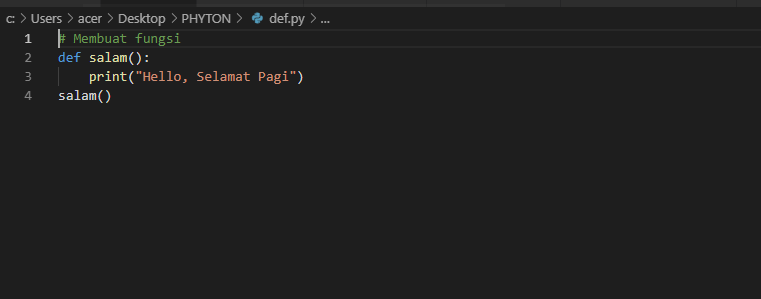
\includegraphics[width=8cm]{figure/satu.PNG}}
\end{figure}

\section{Package}
\paragraph{}
package merupakan sekumpulan file atau modul yang terdapat sebuah fungsi yang dapat dijalankan. Cara pemanggilannya yaitu sebagai berikut :
\begin{figure}[h]
\centerline{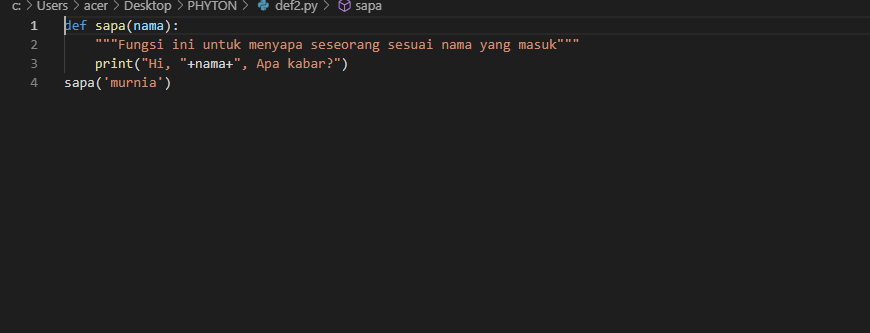
\includegraphics[width=8cm]{figure/2.PNG}}
\end{figure}

\section{Class}
class merupakan blueprint dari sebuah object.
\begin{figure}[h]
\centerline{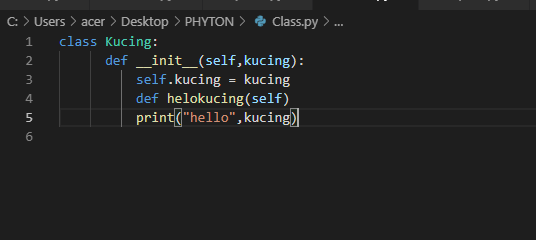
\includegraphics[width=8cm]{figure/a.PNG}}
\end{figure}
\subsection{Object}
object merupakan bagian dari program yang berada dalam sebuah class.
\begin{figure}[h]
\centerline{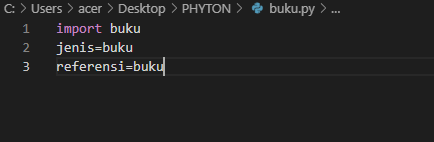
\includegraphics[width=8cm]{figure/4.PNG}}
\end{figure}
\subsection {Atrribute}
attribute merupakan bagianyang dimiliki oleh sebuah class.
\begin{figure}[h]
\centerline{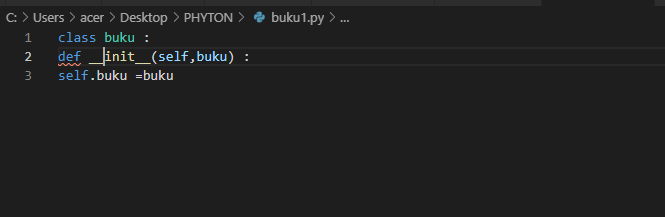
\includegraphics[width=8cm]{figure/5.PNG}}
\end{figure}
\newpage \subsection {Method}
method merupakan fungsi atau program yang ada pada dalam sebuah class.

\begin{figure}[h]
\centerline{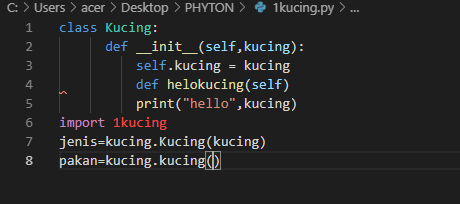
\includegraphics[width=8cm]{figure/6.PNG}}
\end{figure}

\section{Penggunaan Library}
contoh membuat cara sebuah library:
\begin{figure}[h]
\centerline{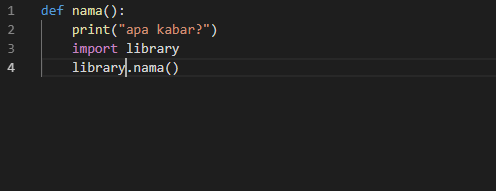
\includegraphics[width=8cm]{figure/3.PNG}}
\end{figure}

\section{Pemakaian Package From Kalkulator Import Penambahan}
\par Sebelum mengimport maka terlebih dahulu kita membuat package perhitungan.
\begin{figure}[h]
\centerline{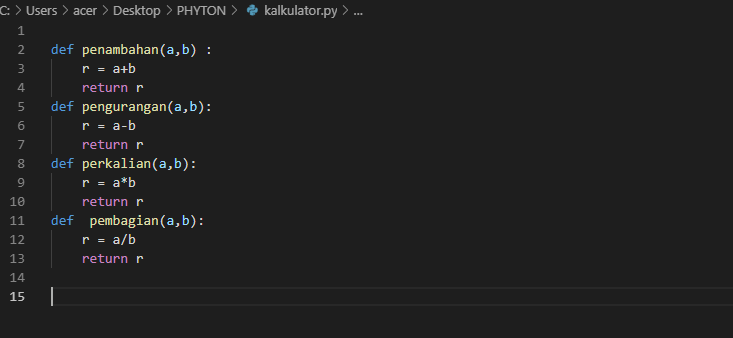
\includegraphics[width=8cm]{figure/f.PNG}}
\end{figure}

\begin{figure}[h]
\centerline{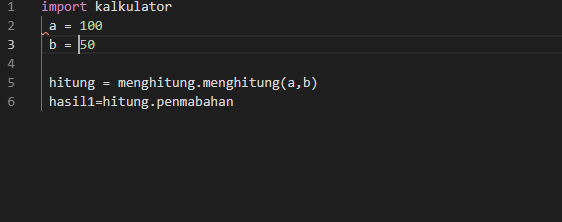
\includegraphics[width=8cm]{figure/g.PNG}}
\end{figure}

\section{Pemanggilan Library dalam Sebuah Folder}
untuk memanggil sebuah library dalam sebuah folder yang pertama yang harus di panggil adalah nama foldernya terlebih dahulu lalu dilanjutkan dengan mengimport library contoh :
\begin{figure}[h]
\centerline{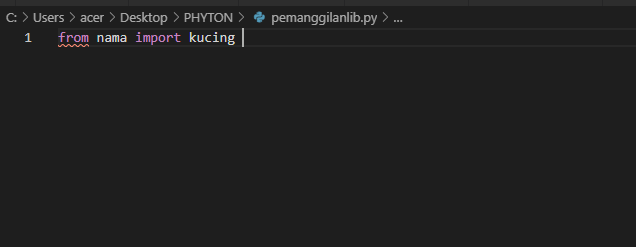
\includegraphics[width=8cm]{figure/d.PNG}}
\end{figure}



\section{Pemanggilan Class dalam Sebuah Folder}
untuk memanggil sebuah class yang pertama yang harus dipanggil adalah folder kita perlu menuliskan foldernyalalu dilanjutkan dengan mengimport nama class nya, contoh :
\begin{figure}[h]
\centerline{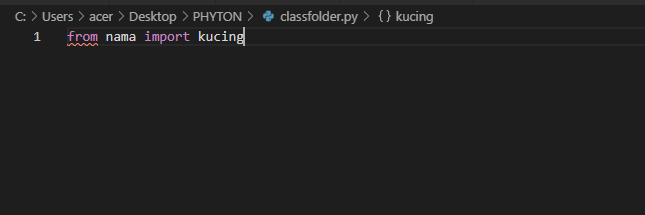
\includegraphics[width=8cm]{figure/e.PNG}}
\end{figure}

\newpage\section{Keterampilan Pemrograman}
\subsection{}
\begin{figure}[h]
\centerline{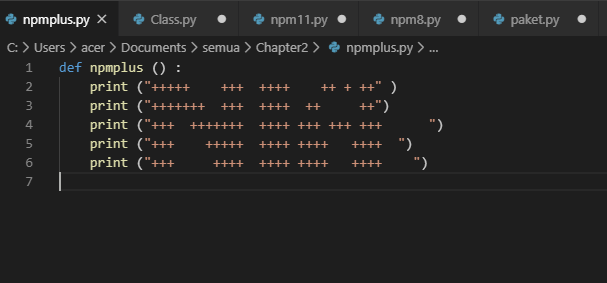
\includegraphics[width=5cm]{figure/1.PNG}}
\end{figure}
\subsection{}
\begin{figure}[h]
\centerline{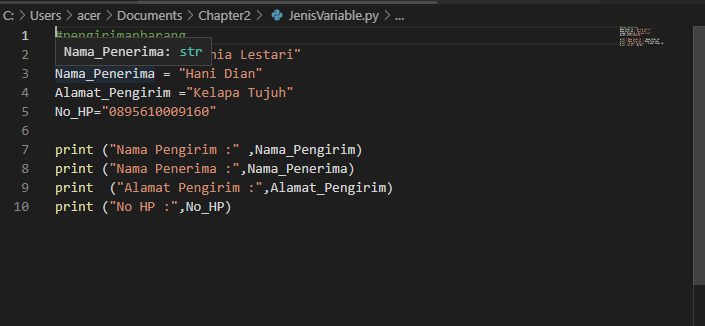
\includegraphics[width=5cm]{figure/A.PNG}}
\end{figure}
\subsection{}
\begin{figure}[h]
\centerline{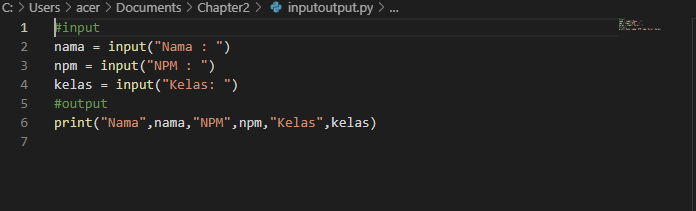
\includegraphics[width=5cm]{figure/B.PNG}}
\end{figure}
\newpage\subsection{}
\begin{figure}[h]
\centerline{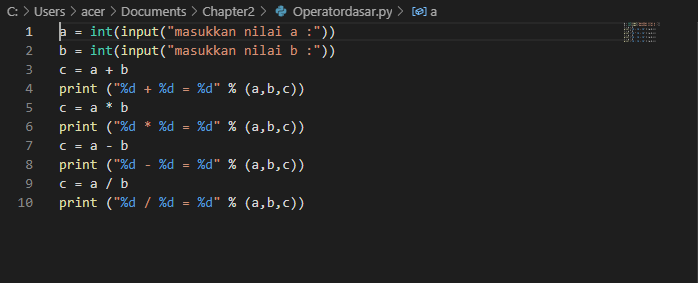
\includegraphics[width=5cm]{figure/C.PNG}}
\end{figure}
\subsection{}
\begin{figure}[h]
\centerline{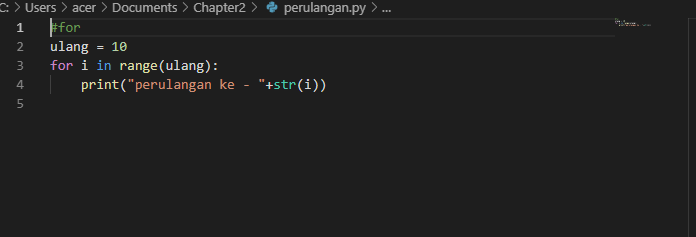
\includegraphics[width=5cm]{figure/D.PNG}}
\end{figure}
\newpage\subsection{}
\begin{figure}[h]
\centerline{\includegraphics[width=5cm]{figure/E.PNG}}
\end{figure}
\subsection{}
\begin{figure}[h]
\centerline{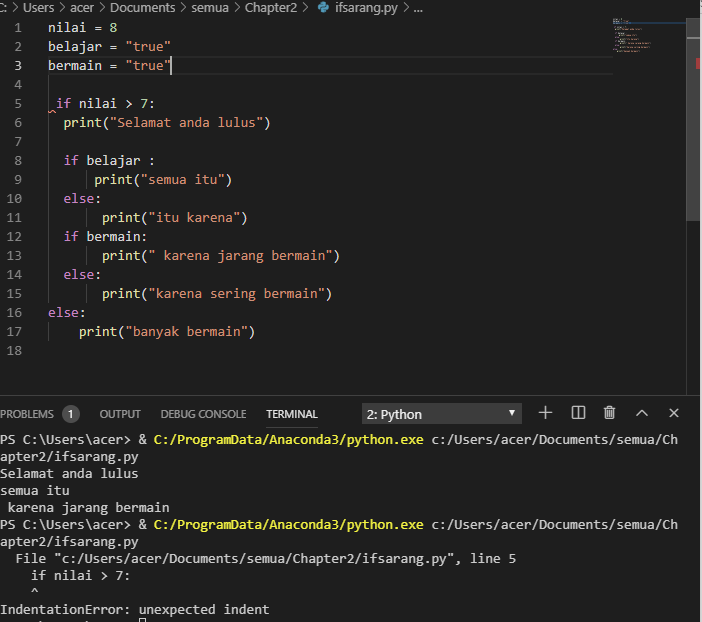
\includegraphics[width=5cm]{figure/F.PNG}}
\end{figure}
\newpage\subsection{}
\begin{figure}[h]
\centerline{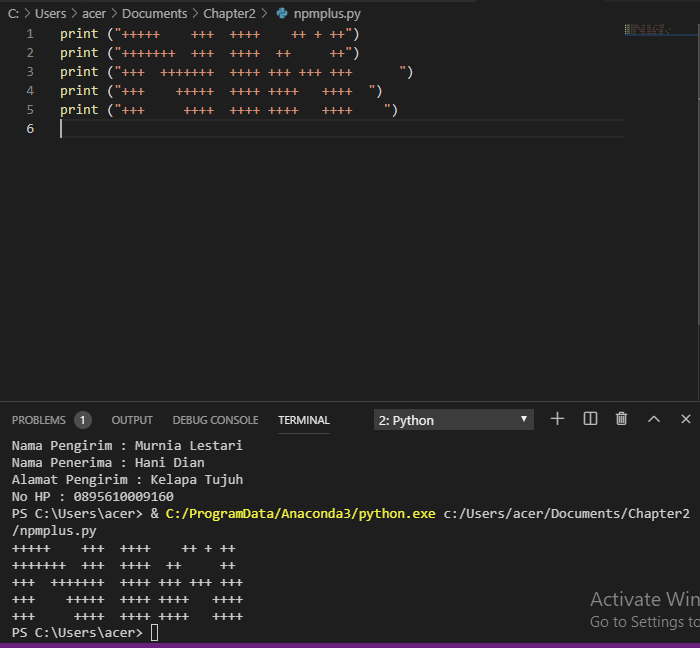
\includegraphics[width=5cm]{figure/G.PNG}}
\end{figure}
\subsection{}
\begin{figure}[h]
\centerline{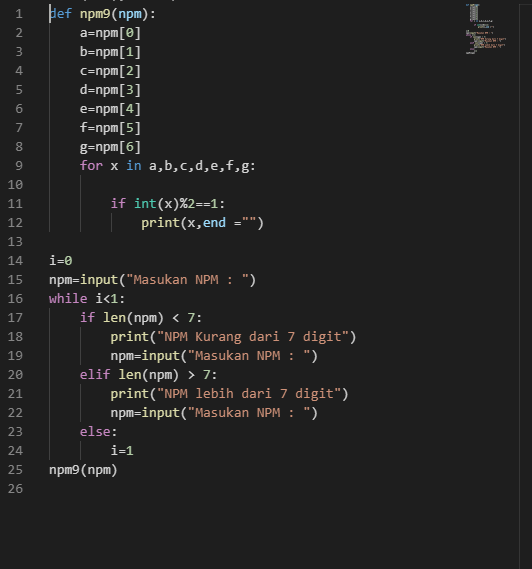
\includegraphics[width=5cm]{figure/H.PNG}}
\end{figure}
\newpage\subsection{}
\begin{figure}[h]
\centerline{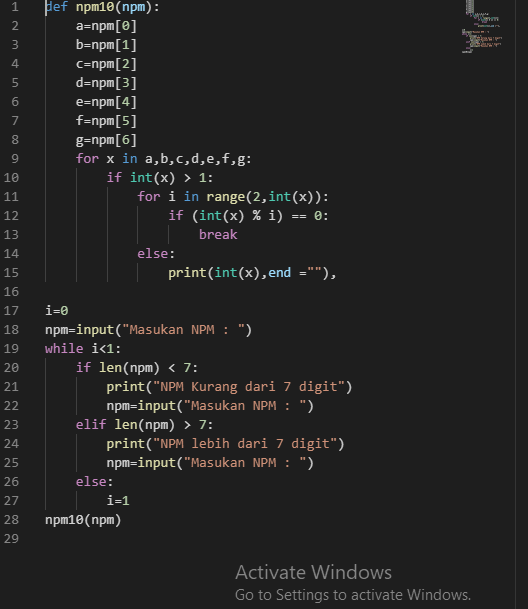
\includegraphics[width=5cm]{figure/I.PNG}}
\end{figure}
\subsection{}
\begin{center}
{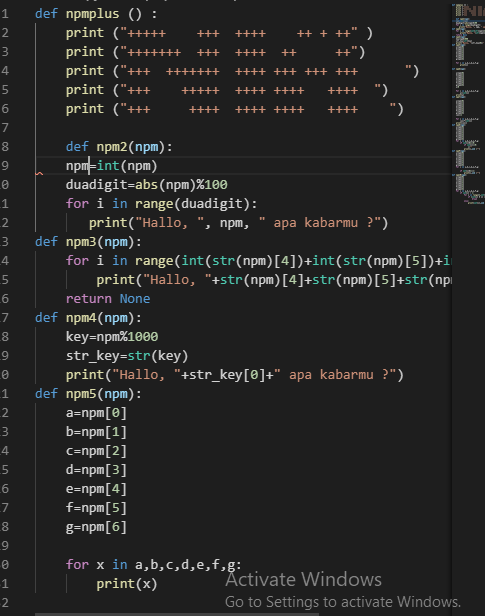
\includegraphics[width=5cm]{figure/K1.PNG}}
{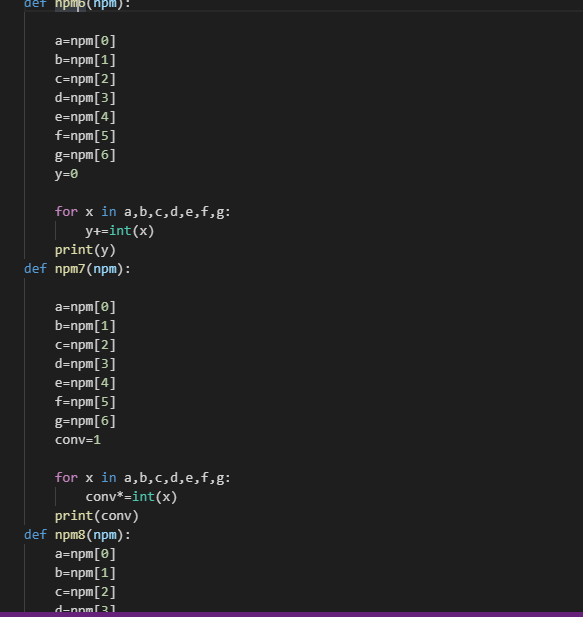
\includegraphics[width=5cm]{figure/K2.PNG}}
{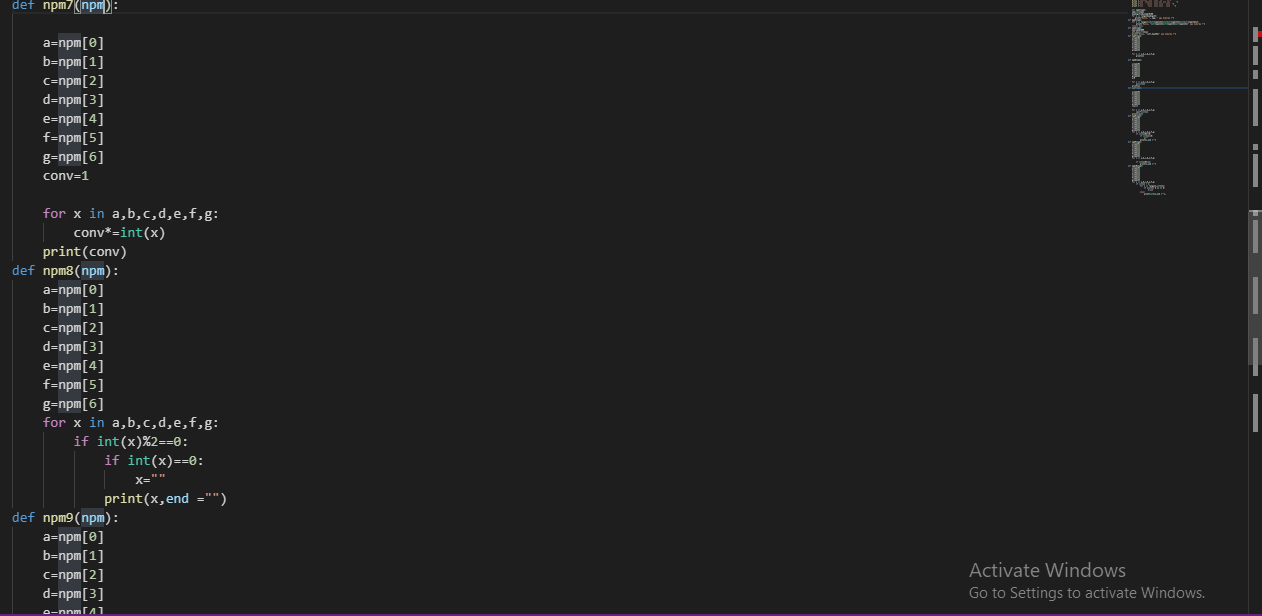
\includegraphics[width=5cm]{figure/K3.PNG}}
{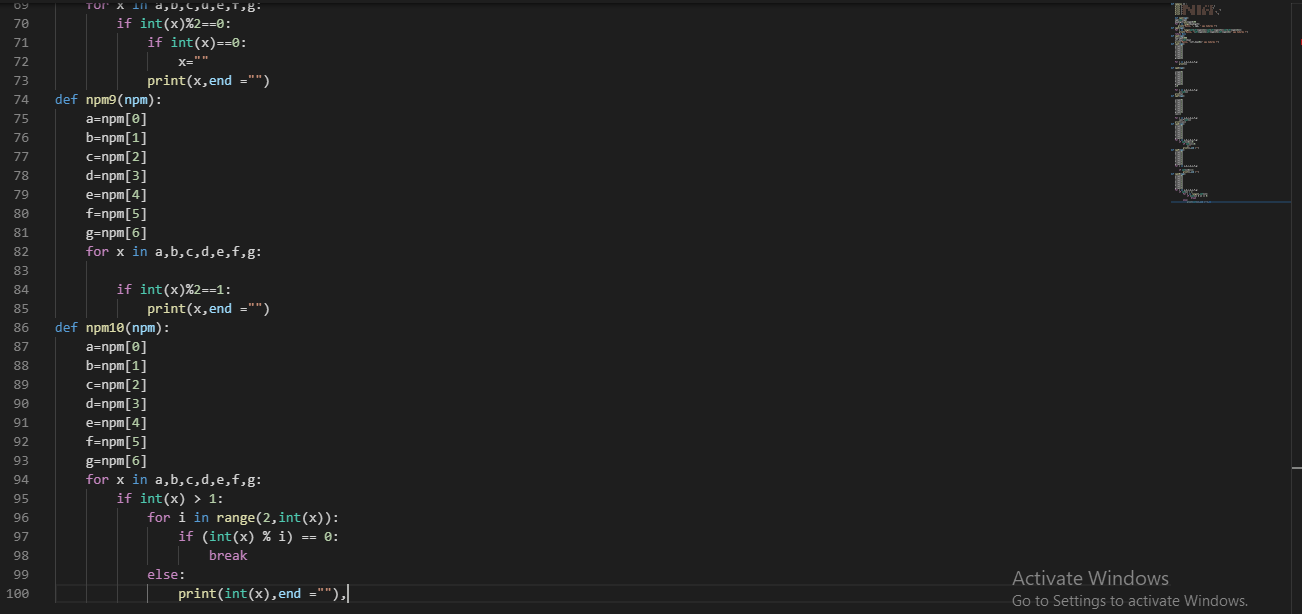
\includegraphics[width=5cm]{figure/K4.PNG}}
\end{center}
\newpage\subsection{}
\begin{figure}[h]
\centerline{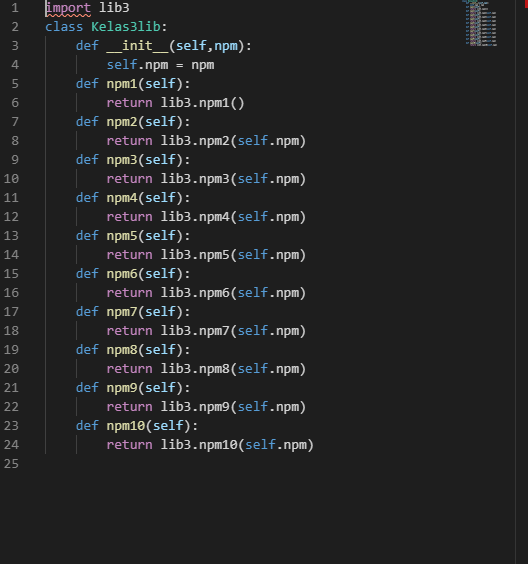
\includegraphics[width=5cm]{figure/J.PNG}}
\end{figure}
\par MAIN.py

\begin{figure}[h]
\centerline{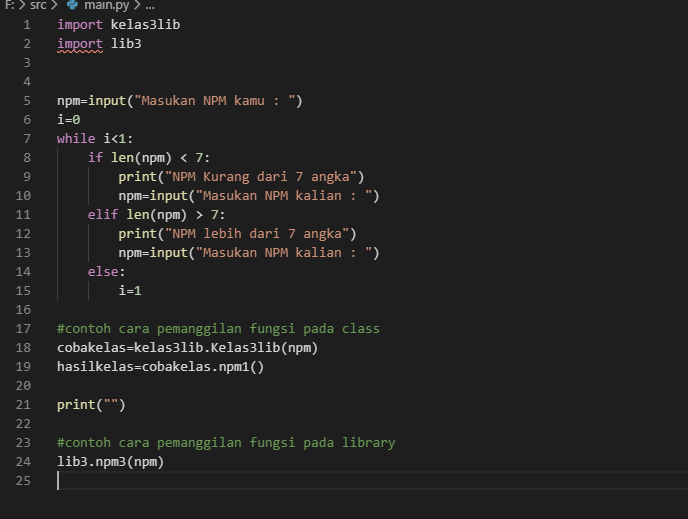
\includegraphics[width=5cm]{figure/M.PNG}}
\end{figure}
\section{Keterampilan Penanganan Error}
\par Seperti dibawah ini error terjadi karena pemanggilan variable yang tidak tepat
\begin{figure}[h]
\centerline{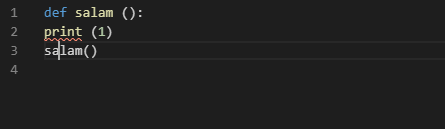
\includegraphics[width=5cm]{figure/N.PNG}}
\end{figure}
\newpage\par Cara mengatasi error diatas adalah try dan except untuk menangkap kesalahan yang ada
\begin{figure}[h]
\centerline{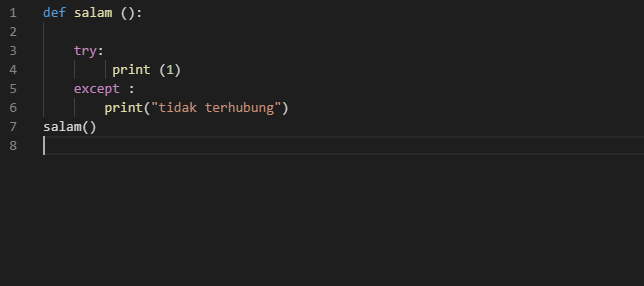
\includegraphics[width=5cm]{figure/O.PNG}}
\end{figure}
\end{document}
